













%\chapter{The FACET E210 Experiment}
In 2014 the experimental campaign  for demonstrating the proof-of-concept of Trojan Horse injection (see \ref{sec:Theory_TrojanHorse}) started at the Facility for Advanced Accelerator Experimental Tests (FACET) at the SLAC national laboratory as the experiment E210. It was a collaborative effort with researchers from the University of Hamburg, University of California Los Angeles (UCLA), University of Strathclyde Glasgow and Radiabeam technology with a devoted support from the SLAC personnel. The FACET experiments had to be designed to be non-excluding, which led to a fruitful joint learning process between several groups.
It is fair to say that E210 was one of the most complex and accuracy-wise most demanding experiments conducted so far at FACET. 
Several steps were required in improving the overall setup, until the experiment was eventually successful.
The most crucial obstacles to overcome were timing and alignment between two laser arms and the electron beam.
The timing requirements between the electron beam and the pre-ionization laser are rather soft as long as the pre-ionization occurs before the arrival of the electron beam an with a timing difference less then the recombination time (ns-µs range). However, proper control over relative time-of-arrival between the injection laser and the electron beam required - in principal - control over timing on the order of $10\ \mathrm{fs}$. With an expected timing jitter in the range of $200\ \mathrm{fs}$ the best solution here was to accurately measure the relative TOA with an electro-optical sampling (described in\ref{sec:EOS}) to determine the injection properties from the data, rather than hope for live-control. 
For finding the synchronization ($t_0$) as well as fine-alignment between electron beam and injection laser, a newly observed effect on the plasma glow described in \ref{sec:Plasma_Glow} was measured and applied.

\section{The FACET experimental setup}
\subsection{Laser energy calibration}
The FACET laser system ...
The energy that can be used on target of the OAP is controlled at two points in the laser-beamline.
At each point a cube-polarizer is surrounded by two  $\lambda/2$-waveplates, where the upstream one is motorized.
The main energy waveplate is located in the laser-room and the probe-energy waveplate is located in the tunnel area shortly after the split between main laser path and probe laser path at the main sampler, which means that the probe laser energy is determined by both waveplate settings while the main laser energy is set by the main laser energy waveplate only. From the power-meter in the laser-room, that measures shot-by-shot laser pulse energy, all the way down to the tunnel a variety of optical components are used until the laser is finally focused onto the 
The typical shot-to-shot laser energy jitter  is $\approx 5 \%$ FWHM.

Manta Cameras: \cite{GigE125_datasheet}

\begin{figure}[htbp]
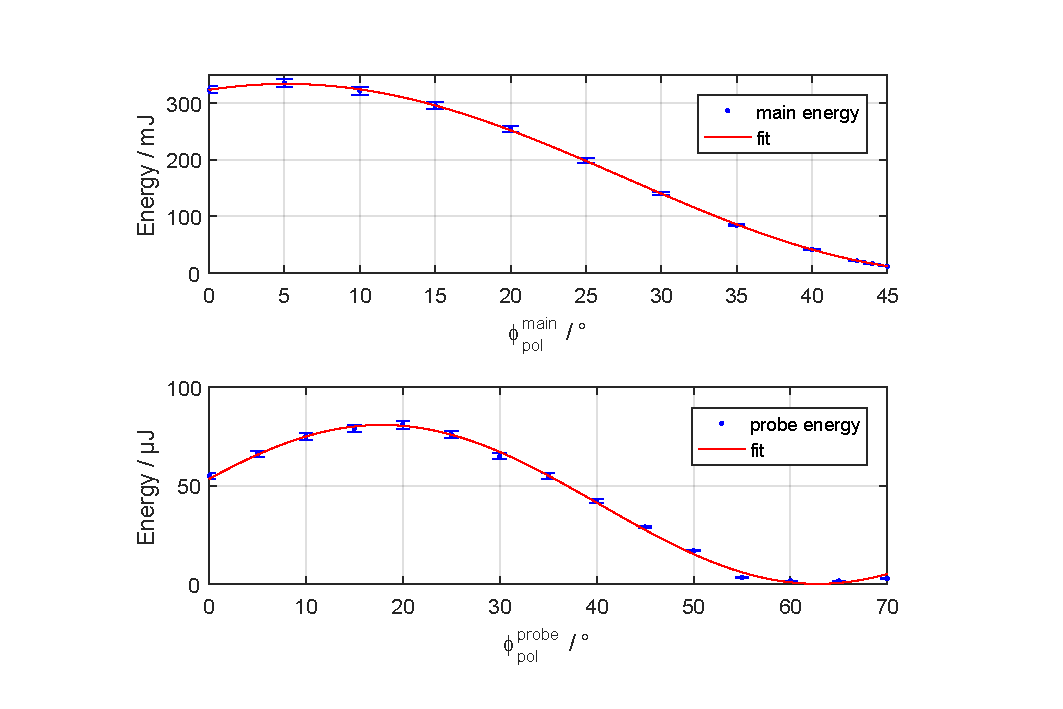
\includegraphics[width=0.9\textwidth]{experiment/images/edited/waveplate_calibration.pdf}
\caption{Laser energy calibration for main energy waveplate (upper plot) and probe energy waveplate (lower plot)}
\label{img:LaserEnergyCalib}
\end{figure}

All measured losses in optical components combined with the fitted functions for the waveplate energies (see figure \ref{img:LaserEnergyCalib}) combined give the on target energy applicable by axilens and OAP respecively.
\begin{align*}
 W_\mathrm{Laser}^\mathrm{OAP} &= W_\mathrm{Laser}^\mathrm{Laserroom}\times 1.25\times10^{-2}\\ 
 &\times\big( 0.994 \cos^2((\phi_{pol}^{main}+66.9\degree)) +1.16\times 10^{-3}\big)\\
  &\times \big(0.998 \cos^2((\phi_\mathrm{pol}^\mathrm{probe}-17.8\degree )) +1.62\times 10^{-3}\big)
\end{align*}

\begin{align}
 W_\mathrm{Laser}^\mathrm{Axilens} &= W_\mathrm{Laser}^\mathrm{Laserroom}\times 0.253\\
  &\times\big( 0.994 \cos^2((\phi_\mathrm{pol}^\mathrm{main}+66.9\degree)) +1.16\times 10^{-3}\big)\\
\end{align}
This means that for a typical laser energy output of $500\, \mathrm{mJ}$ a maximum energy of $6.2\, \mathrm{mJ}$ on OAP target and $125.9\,\mathrm{mJ}$ on axilens could be used.


\section{Electro Optical Sampling (EOS)}
\label{sec:EOS}
In order to measure the relative time-of-arrival between electron bunch and laser pulse, a non-destructive shot-to-shot diagnostic was necessary. Electro-optical sampling is an excellent choice for sub-picosecond electron bunches \cite{YanX_EOS_PRL2000}.
An externally applied electric field to crystals like GaP and ZnTe induces a birefringence in the optical axis of the material. This effect is called the pockels, or electro-optic effect. In this experiment the crystal is  located in close proximity (few mm distance) to the electron beam axis. Due to the high $\gamma_\mathrm{b} \approx 42000$ , the beam electric field is strongly lorenz-contracted and can be assumed to temporally only extend for the length of the electron beam. Consequently the electric field applied to the crystal and with that the induced birefringence are only active while the electron beam passes by the crystal. 
A linear polarized laser pulse, traversing the crystal at the same time will change its polarization and is analyzed by a polarizing filter.

The crystal plate is oriented perpendicular to the electron beam axis to minimize temporal overlap and the laser has an $\approx 40°$ angle with the electron beam which enables a correlation between signal position i.e. the part of the laser with rotated polarization and relative timing.

The entire ladder supports a YAG crystal to find the electron beam axis, a $500\ \mathrm{µm}$ thick ZnTe for broad timing scans and GaP with $100\ \mathrm{µm}$ thickness for fine resolution.
A detailed description of the physics involved in the application of electro-optical crystals as TOA and bunch length diagnostic can be found in \cite{BerndSteffenPhD}.

\begin{figure}[htbp]
\includegraphics[width=0.5\textwidth]{experiment/images/edited/EOS_setup.pdf}
\caption{Setup of upstream electro-optical sampling inside the picnic basket chamber. Electron beam (green) and EOS laser (red) co-propagate in a small angle }
\label{img:EOS_Setup}
\end{figure}
\begin{figure}
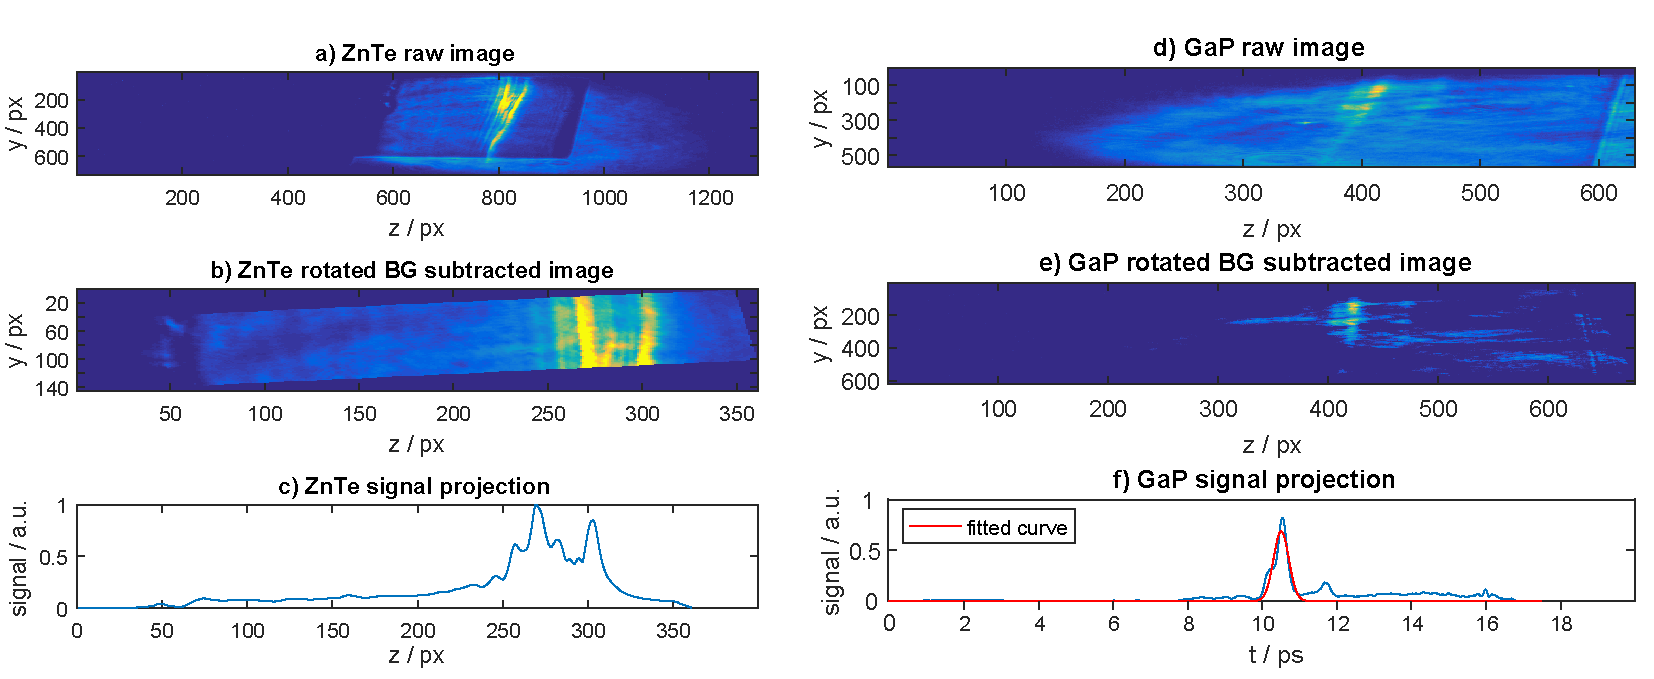
\includegraphics[width=1.0\textwidth]{experiment/images/edited/EOS_Signal.pdf}
%\caption{}
\label{img:EOS_ZnTe}
\end{figure}


%\section{Torch kick}
%\begin{figure}[htbp]
%\includegraphics[width=0.9\textwidth]{experiment/images/raw/Torch_rollscan.pdf}
%\caption{'test'}
%\label{img:TochKick}
%\end{figure}
\newpage
\section{Ionization test}

\section{Plasma glow diagnostic}
\label{sec:Plasma_Glow}
One huge advantage of the hydrogen FACET setup compared to the oven setup is that now several view ports allow for observing the interaction or \ref{Facet_setup}.

The plasma glow diagnostic as a very simple tool, that turned out to be extremely helpful in controlling the 
alignment and synchronization of the experimental setup. The main idea is to have a camera integrate over the recombination light. It was observed that this 

\begin{figure}[htbp]
\includegraphics[width=1\textwidth]{experiment/images/raw/PlasmaGlow_20384_scatter.pdf}
\caption{Relative electron beam to injection laser timing scan. The pixel counts measured by the cube 3 vertical camera with a 656$\pm$10 nm  band-pass filter are sorted by the EOS. evaluation.}
\label{img:PlasmaGlowTimingOAP_H2He}
\end{figure}

Figure \ref{img:PlasmaGlowTimingOAP_H2He} shows the plasma glow accumulated intensity at the wavelength 656$\pm$10 nm , sorted by relative time-of-arrival between electron beam as measured by the EOS. The transition between a situation where the injection laser arrives earlier than the electron beam and vice versa is around $1\ \mathrm{ps}$ wide, which sufficiently fulfills the requirements to find a range of synchronization as the total range of the EOS crystal is around 20 ps ???.
During the data acquisition the electron beam charge was $3.1\pm \ 0.17\ \mathrm{nC}$. 

\begin{figure}[htbp]
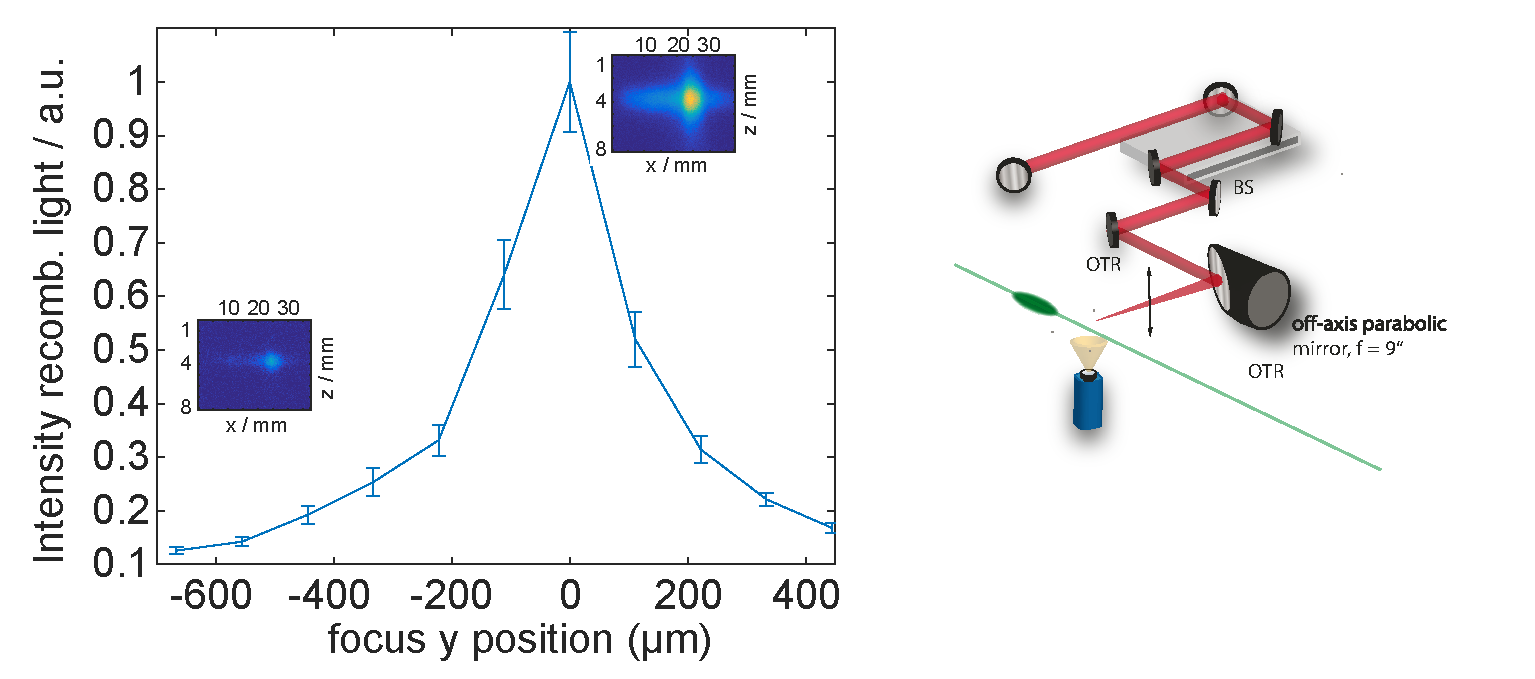
\includegraphics[width=0.5\textwidth]{experiment/images/edited/Plasma_Glow_roll.pdf}
\caption{Plasma glow in 4 torr $\mathrm{H}_2$ measured by vertical camera in cube 3. The injection laser off-axis parabola roll is scanned. The vertical plasma position is evaluated by the focus diagnostic.}
\label{img:PlasmaGlowRoll}
\end{figure}



\subsection*{Result:}
With the 
